\chapter{Modeller} \label{chap:klasser}

I dette kapitel vil klasserne i modellaget blive beskrevet.

\begin{figure}[H]
  \centering
  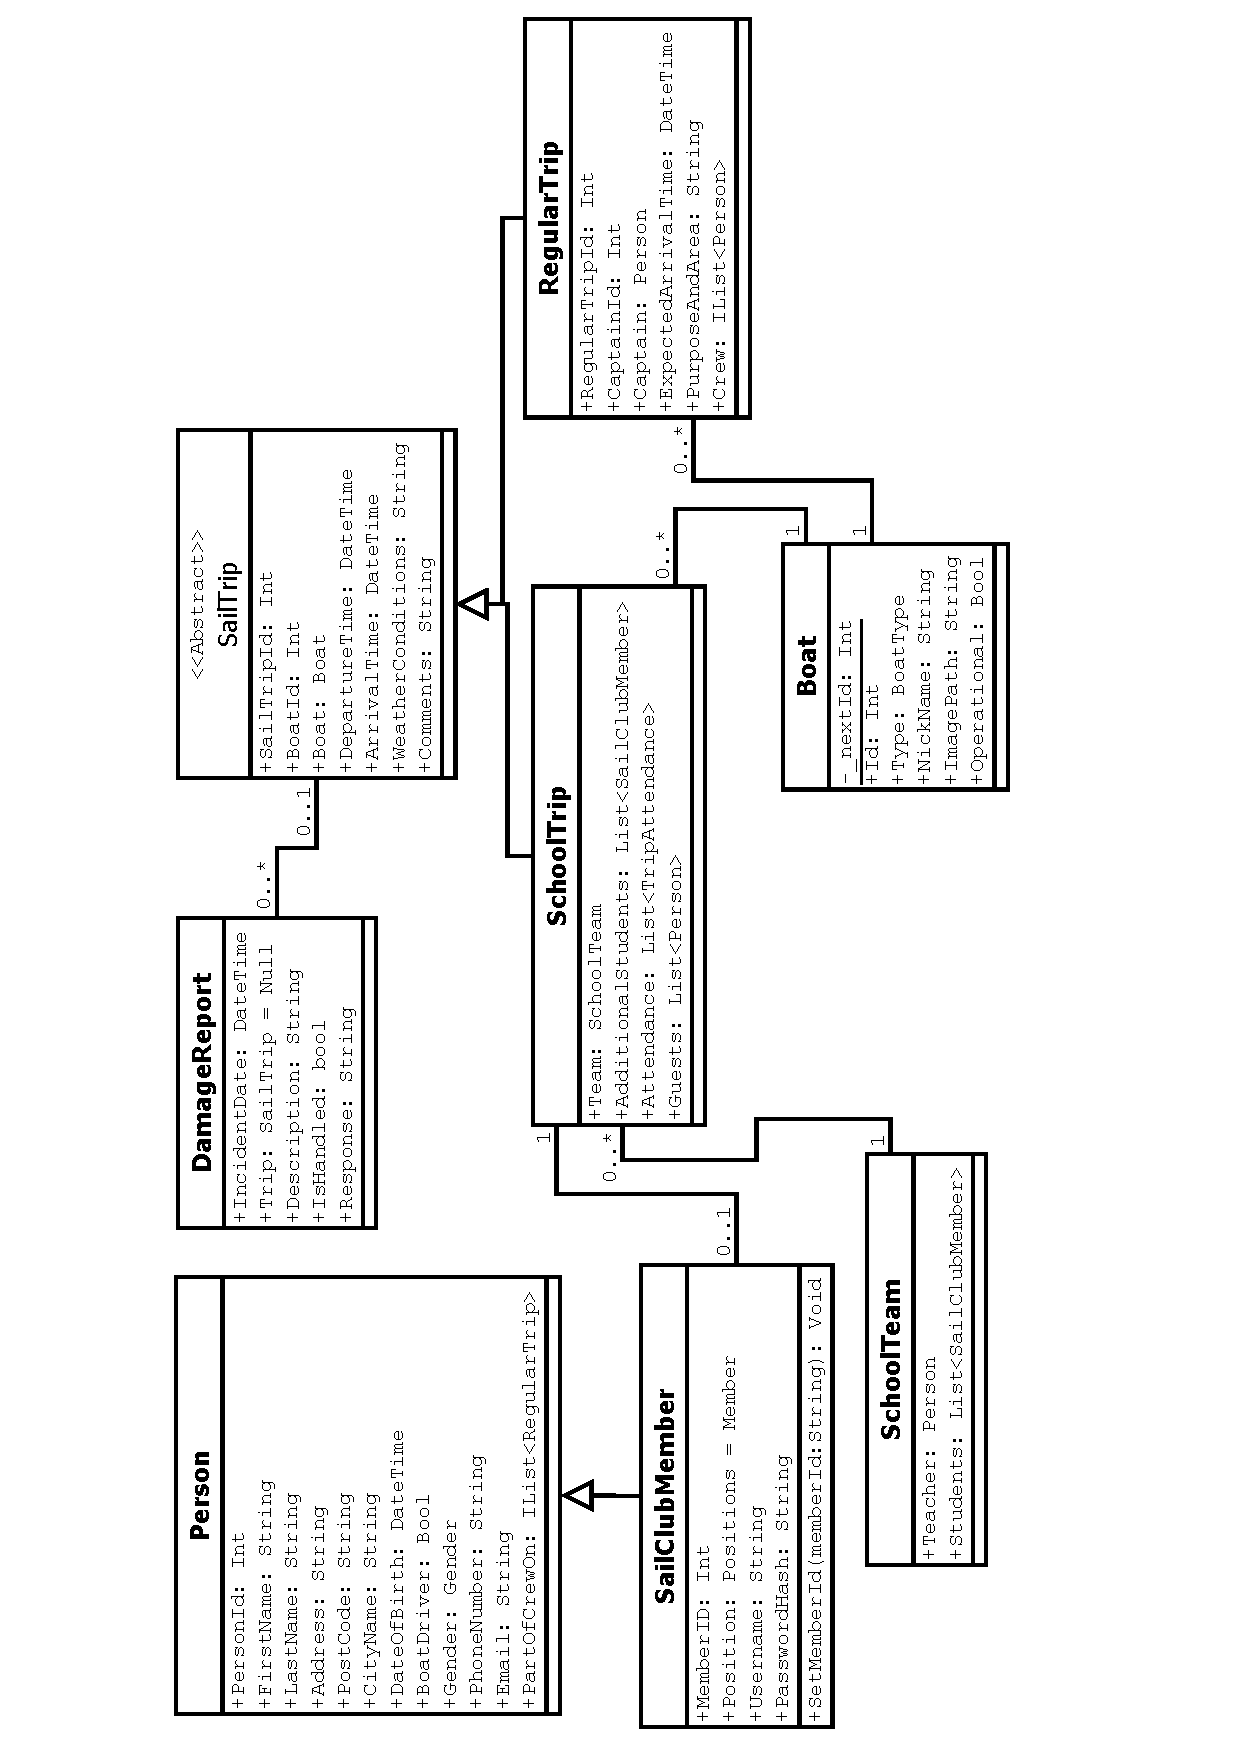
\includegraphics[width=0.70\textwidth]{images/flowcharts/UML.pdf}
  \caption{UML-diagram over klasserne i projektets program}\fxnote{Caspar: det er vel ikke projektets program? evt. ``UML-diagram over klasserne i programmet'' bare}
  \label{img:UML}
\end{figure}

\subsection*{Klasse: Person} \fxnote{Troels: Vi ændrede Felter til formål på et tidspunkt, men flere starter nu med felter?}
\fxnote{Nikolaj: En reference i starten til UML-diagrammet, i stedet for ved hver klasse? Bedre brug af section/subsections somehow, måske skal afsnit tallene også bare fjernes fra person klassen}
\textbf{Formål:}
I personklassen findes felter, som indeholder informationer vedrørende personen. Felterne ses på \myref{img:UML}.

\textbf{Metoder:}
Personklassen har overrided \textbf{ToString()}, som returnerer \textbf{FullName}.\fxnote{Søren) : Overskrevet??}

\textbf{Anvendelse:}
Personklassen bruges til at repræsentere alle personer i systemet. 
Gæster repræsenteres direkte som instanser af personklassen. 
Sejlklubbens medlemmer repræsenteres som subklasser af personklassen. 

\subsection*{Klasse: SailClubMember}

\textbf{Formål:}
SailClubMember nedarver fra personklassen og tilføjer felter, som er vigtige for at repræsentere hvert medlem.
Disse felter kan ses på \myref{img:UML}.

\textbf{Position} feltet angiver hvilken rang, og dermed rettigheder, som et sejlklubmedlem har. 
Dette repræsenteres ud fra en enumeration.

\textbf{Anvendelse:}
SailClubMember bruges til at danne instanser af alle sejlklubbens medlemmer. \fxnote{Troels: Bortset fra studerende, som er en instans af studentmember som nedarver herfra}

\subsection*{Klasse: StudentMember}
\textbf{Formål:}
Klassen StudentMember indeholder informationer om, hvilke læringsmål eleven har udført i forbindelse med sejlerskolen. 

\textbf{Anvendelse:}
Klassen StudentMember nedarver fra SailClubMember og bruges til at repræsentere eleverne i sejlklubben.

\subsection*{Klasse: Team}

\textbf{Formål:}
Klassen Team indeholder informationer om et vilkårligt hold.\fxnote{Tristan: Måske et sejlskolehold?}
Samtidigt inderholder den både en liste over elever og lektioner.

\textbf{Anvendelse:}
Team anvendes til at samle en gruppe elever i sejlerskolen.
Denne samling gør det muligt at håndtere eleverne på holdet på samme tid.

\subsection*{Klasse: SailTrip og RegularSailTrip}

I en tidlig designstruktur var det tænkt at programmet skulle indeholde flere forskellige typer af sejlture, og derfor blev SailTrip-klassen skabt som værende superklasse for sejltursklasser. 
Senere blev ideen om at have flere typer sejlture ændret, og i stedet blev der valgt, at der kun skulle være én sejlturstype. 
SailTrip-klassen er dog bibeholdt i tilfælde af videre udbygning af programmet.
Dog findes der enkelte felter i klasserne, som overlapper hinanden lidt, men felter er også bibeholdt i tilfælde af udbygning til flere typer sejlture.

\textbf{Formål:}
Felterne i klasserne indeholder de nødvendige informationer for at kunne reservere en båd.
Feltet WeatherConditions er placeret her, men udfyldes først i logbogen, da det er sejlturen, og ikke logbogen, som havde et vejrforhold.
Desuden indeholder klassen SailTrip en reference til en logbog, som er den logbog, som udfyldes senere i forbindelse med sejlturens afslutning.

\textbf{Anvendelse:}
SailTrip-klassen anvendes kun som superklasse for RegularTrip-klassen. 
Hver reservation er en instans af klassen RegularTrip, dette gælder også reservationer for sejlerskolens lektioner.

\subsection*{Klasse: Event}

\textbf{Formål:} \fxnote{Troels: Er dette et formål?}
Klassen indeholder felter, som giver en beskrivelse af, hvornår og hvad begivenheden går ud på. 

\textbf{Anvendelse:}
En instans af eventklassen repræsenterer en begivenhed. 
Det behøver ikke at være en sejlrelateret begivenhed.
\fxnote{(Søren): " En instans af evenklassen, repræsenterer en begivenhed, der ikke nødvendigvis er sejlrelateret}

\subsection*{Klasse: Logbook}

\textbf{Formål:}
Klassen logbook indeholder de nødvendige informationer, som bruges til postsejlads dokumentation, som beskrevet i \myref{subsec:bådudlån}.

\textbf{Anvendelse:}
En instans af klassen Logbook findes på hver sejltur. 
Den udfyldes af personen, som har foretaget reservationen, efter sejladsens fuldførelse. 

\subsection*{Klasse: Lecture}

\textbf{Formål:}
Klassen Lecture indeholder information vedrørende en undervisning. 

\textbf{Anvendelse:}
Denne klasse bruges, når der reserveres en båd til sejlerskolen og samtidigt til at registrere, hvilke læringsmål som blev udført på turen. 

\fxnote{Nogle steder har vi sat et myref ind til UML'en. Skal vi gøre det hele tiden ? Hvordan skal vi organisere det kapitel??}
